%%%%%%%%%%%%%%%%%%%%%%%%%%%%%%%%%%%%%%%%%%%%%%%%%%%%%%%%%%%%%%%%%%%%%%
% 
% 	Template for Producing ASP-DAC 2018 Proceedings
% 
%%%%%%%%%%%%%%%%%%%%%%%%%%%%%%%%%%%%%%%%%%%%%%%%%%%%%%%%%%%%%%%%%%%%%%
% History
% ??/??/?? Designed by Hiroaki Kunieda (ASP-DAC '97 Publication Chair)
% 09/22/97 Modified and small bug fixed by Masaharu Imai 
% 	   (ASP-DAC '98 Publication Chair)
% 11/02/98 Modified by Tsuyoshi Isshiki
% 	   (ASP-DAC 2000 TPS Secretary)
% 7/24/00 Modified by Kiyoharu Hamaguchi
% 	   (ASP-DAC 2001 Publication chair)
% 6/18/02 Modified by Kazutoshi Kobayashi
% 	   (ASP-DAC 2003 Publication Co-Chair)
% 5/27/03 Modified by Kiyoharu Hamaguchi
% 	   (ASP-DAC 2004 TPC secretary)
% 6/10/03 Modified by Kazutoshi Kobayashi for Latex2e
% 	   (ASP-DAC 2004 Publication Co-Chair)
% 6/01/05 Modified by Nozomu Togawa
% 	   (ASP-DAC 2006 Publication Chair)
% 6/01/06 Modified by Hiroyuki Ochi
% 	   (ASP-DAC 2007 Publication Chair)
% 5/30/08 Modified by Nozomu Togawa
% 	   (ASP-DAC 2009 Publication Co-Chair)
% 4/30/10 Modified by Masashi Imai
% 	   (ASP-DAC 2011 Publication Chair)
% 3/20/12 Modified by Masashi Imai
% 	   (ASP-DAC 2013 Publication Chair)
% 5/01/14 Modified by Masashi Imai
% 	   (ASP-DAC 2015 Publication Chair)
% 4/24/16 Modified by Masashi Imai
% 	   (ASP-DAC 2017 Publication Chair)
% 2/06/17 Modified by Jongeun Lee
% 	   (ASP-DAC 2018 Publication Chair)
%%%%%%%%%%%%%%%%%%%%%%%%%%%%%%%%%%%%%%%%%%%%%%%%%%%%%%%%%%%%%%%%%%%%%%
% If you have any problem, please contact ASP-DAC 2018 Publication
% Chair by E-mail at "jlee@unist.ac.kr.''
%%%%%%%%%%%%%%%%%%%%%%%%%%%%%%%%%%%%%%%%%%%%%%%%%%%%%%%%%%%%%%%%%%%%%%
%
\documentclass[twocolumn]{article}
%% If you use dvips and ps2pdf, please use Postscript font 
%% and uncomment the line below.
%%\usepackage{times}
\usepackage[dvipdfmx]{graphicx}
\pagestyle{empty}
%set paper size
%for A4 paper
\topmargin      29mm    %bottom margin 30mm
\oddsidemargin  15mm    %left & right margin 15mm

%for 8 1/2" x 11" paper paper, use the following definition
%\topmargin     17mm    %bottom margin 24mm
%\oddsidemargin 18mm    %left margin 18mm & right margin 17mm

%text sizes
\textwidth  180mm
\textheight 238mm
\columnsep  5.0mm
\parindent  3.5mm

%misc parameters
\headsep 0mm  \headheight 0mm
\footskip 18mm
%\footheight 6mm

%conversion to values for LaTeX
\advance\topmargin-1in\advance\oddsidemargin-1in
\evensidemargin\oddsidemargin

\makeatletter
%as Latex considers descenders in its calculation of interline spacing,
%to get 12 point spacing for normalsize text, must set it to 10 points
\def\@normalsize{\@setsize\normalsize{12pt}\xpt\@xpt
\abovedisplayskip 10pt plus2pt minus5pt\belowdisplayskip \abovedisplayskip
\abovedisplayshortskip \z@ plus3pt\belowdisplayshortskip 6pt plus3pt
minus3pt\let\@listi\@listI}

%interline spaceing and title font for section
\def\section{\@startsection {section}{1}{\z@}{20pt plus 2pt minus 2pt}
{8pt plus 2pt minus 2pt}{\centering\normalsize\sc
\edef\@svsec{\thesection.\ }}}
\def\thesection{\Roman{section}}

%interline spacing and title font for subsection
\def\subsection{\@startsection {subsection}{2}{\z@}{16pt plus 2pt minus 2pt}
{6pt plus 2pt minus 2pt}{\normalsize\sl
\edef\@svsec{\thesubsection.\ }}}
\def\thesubsection{\Alph{subsection}}

%figures/tables captions
\long\def\@makecaption#1#2{
\vskip10pt\begin{center} #1 #2 \end{center}\par\vskip 1pt}
\def\fnum@figure{\raggedright{\footnotesize Fig. \thefigure }.%
\footnotesize}
\def\fnum@table{\footnotesize TABLE \thetable\\\footnotesize\sc}
\def\thetable{\Roman{table}}

\makeatother

%%%%%%%%%%%%%%%%%%%%%%%%%%%%%%%%%%%%%%%%%%%%%%%%%%%%%%%%%%%%%%%%%%%%%%%

\begin{document}
%date not printed
\date{}

%make title
\title{\Large\textbf{Preparation GUIDE for Initial-Submission Manuscript}\\~\\
\large\textbf{
Preparation of Papers in Two-Column Format\\
for the ASP-DAC 2018 (\LaTeX2e version)}}	% Modified by K. Kobayashi 18/06/02

%for single author
%\author{Center the Authors Names Here \\
%Center the Affiliations Here\\
%Center the City, Stats and Country Here\\
%{\small (it is your option if you want your entire address listed)}}

%for two authors
\author{
You must not show authors' names and affiliations in the\\
initial-submission paper. But you had better to make \\
room for the final submission.\\
\\
\\
\\ % To make more spaces just add \\!
}
\maketitle
\thispagestyle{empty}

{\small\textbf{Abstract---
 Abstract is a brief (50-80 word) synopsis of your paper.
The purpose is to provide a quick outline of your
presentation, giving the reader an overview of the
research. It must be fit within the size allowed, which is
about 3 inches or 7.5 centimeters.
}}

\section{Introduction}

These introductions give you basic guidelines for preparing 
initial-submission papers for the ASP-DAC 2018.

The instructions assume that you have computer that can generate a PDF
file. 

These instructions have been prepared in the preferred format. For items
not addressed here, please refer to recent issues of IEEE Transactions
and simulate, as closely as possible.


\section{How to Format the Page}

\subsection{Full-Size Camera-Ready Copy} 

Prepare Initial-Submission paper in full size format, on A4 size or 8 1/2''
$\times$ 11''(21.5cm $\times$ 27.9 cm) paper.

\subsection{Fonts}
The best results will be obtained if your computer word-processor has
several font sizes. Try to follow the font sizes specified in Table I as
best as you can. As an aid to gauging font size, 1 point is about
0.35mm. Use a proportional, serif font such as Times of Dutch Roman.

\begin{table}[tb]
\caption{Fonts for Initial-Submission and Camera-Ready Papers}
\begin{minipage}{8cm}
\def\arraystretch{1.5}\tabcolsep 2pt
\def\thefootnote{a}\footnotesize
\begin{tabular}{l@{~}l@{~~~}l}
\hline
\parbox[c]{7mm}{Font\newline Size} & Style & Text\\
\hline
 14pt&bold     &Paper title\\
 12pt&         &Authors' names\\
 10pt&         &Authors' affiliations, main text, equations,\\[-5pt]
     &         &first letters in section titles\footnotemark[1]\\
 10pt&italic   &Subheddings\\
 ~9pt&bold     &Abstract\\
 ~8pt&         &Section titles\footnotemark[1], table
                names\footnotemark[1], first letters in table\\[-5pt]
     &         &captions\footnotemark[1],
                tables, figure captions, references,\\[-5pt]
     &         &footnotes, text subscripts and superscripts\\
 ~6pt&         &Table captions\footnotemark[1], table superscripts\\
\hline
\end{tabular}
\footnotetext[1]{\scriptsize Uppercase}
\end{minipage}
\end{table}


\subsection{Formats}

In formatting your A4-size paper, set top margin to 29mm (1.14 inches),
bottom margin to 30mm (1.18 inches), left and right margins to 15mm
(0.59 inches) If you are using paper 8 1/2'' $\times$ 11'', set top margin
to 17mm (0.67 inches), bottom margin to 24mm (0.94 inches), left
margin to 18mm (0.71 inches) and right margins to 17mm (0.67 inches). The column
width is 88mm (3.46 inches) with 5mm (0.2 inches) space between the two
columns.

You should left- and right-justify your columns. On the last page of
your paper, try to adjust the lengths of the two columns so that they
are the same. Use automatic hyphenation if you have it and check
spelling. Either digitize or paste down your figures.

%{\bf Number each of you submitted pages at the top, right corner, in
%non-photographic light blue pencil.}


\section{Figures and Tables}
Position figures and tables at the tops and bottoms of columns. Avoid
placing them in the middle of columns. Large figures and tables may
span across both columns. Figure captions should be below the figures;
table captions should be above the tables. Avoid placing figures and
tables before their first mention in the text. Use the abbreviation
``Fig.1'', even at the beginning of a sentence.

\begin{figure}[tb]
 \begin{center}
  \begin{minipage}{\hsize}
   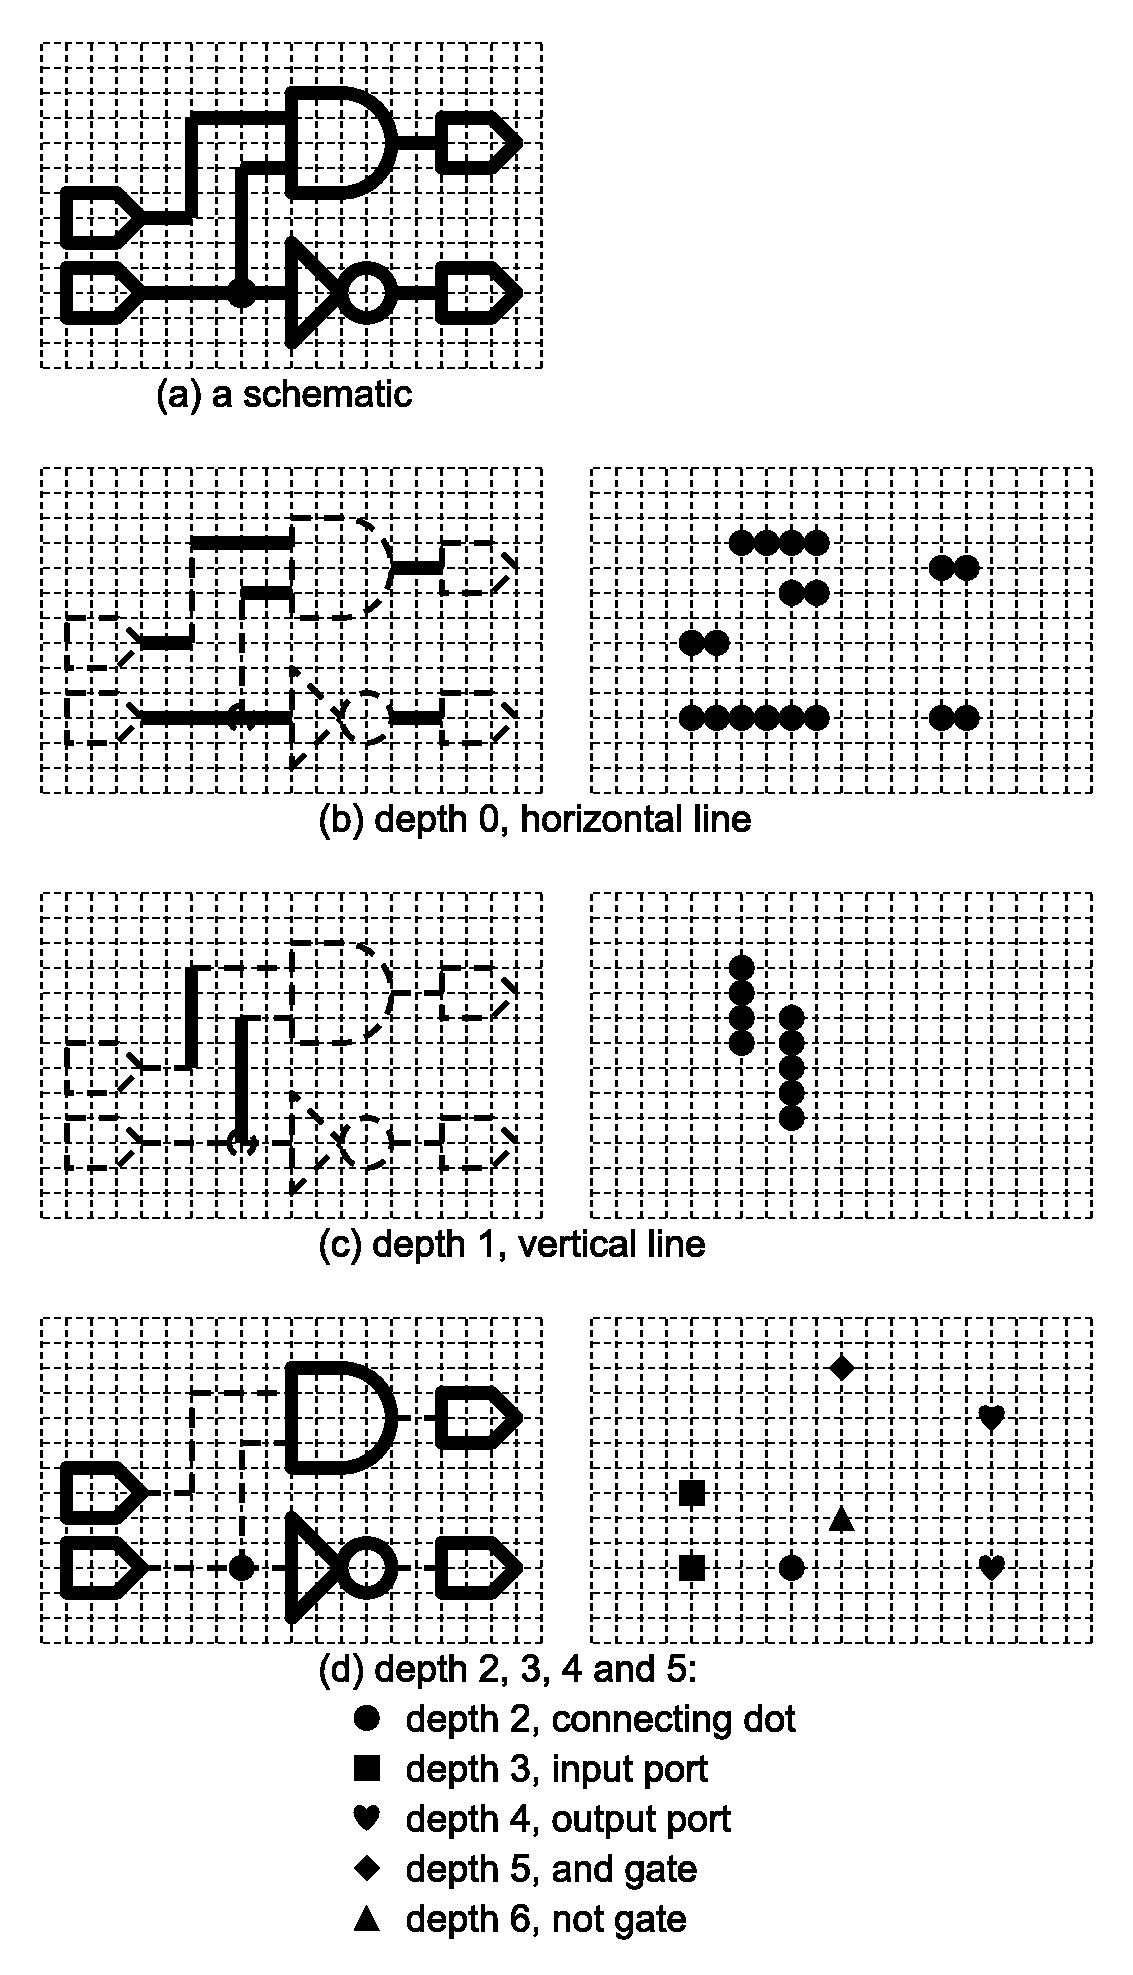
\includegraphics[width=\hsize]{input_encode_03.eps}
   \caption{a way to encode schematic for input vector of neural network}
   \label{fig:input_encode}
  \end{minipage}
 \end{center}
\end{figure}

\begin{figure}[tb]
 \begin{center}
  \begin{minipage}{\hsize}
   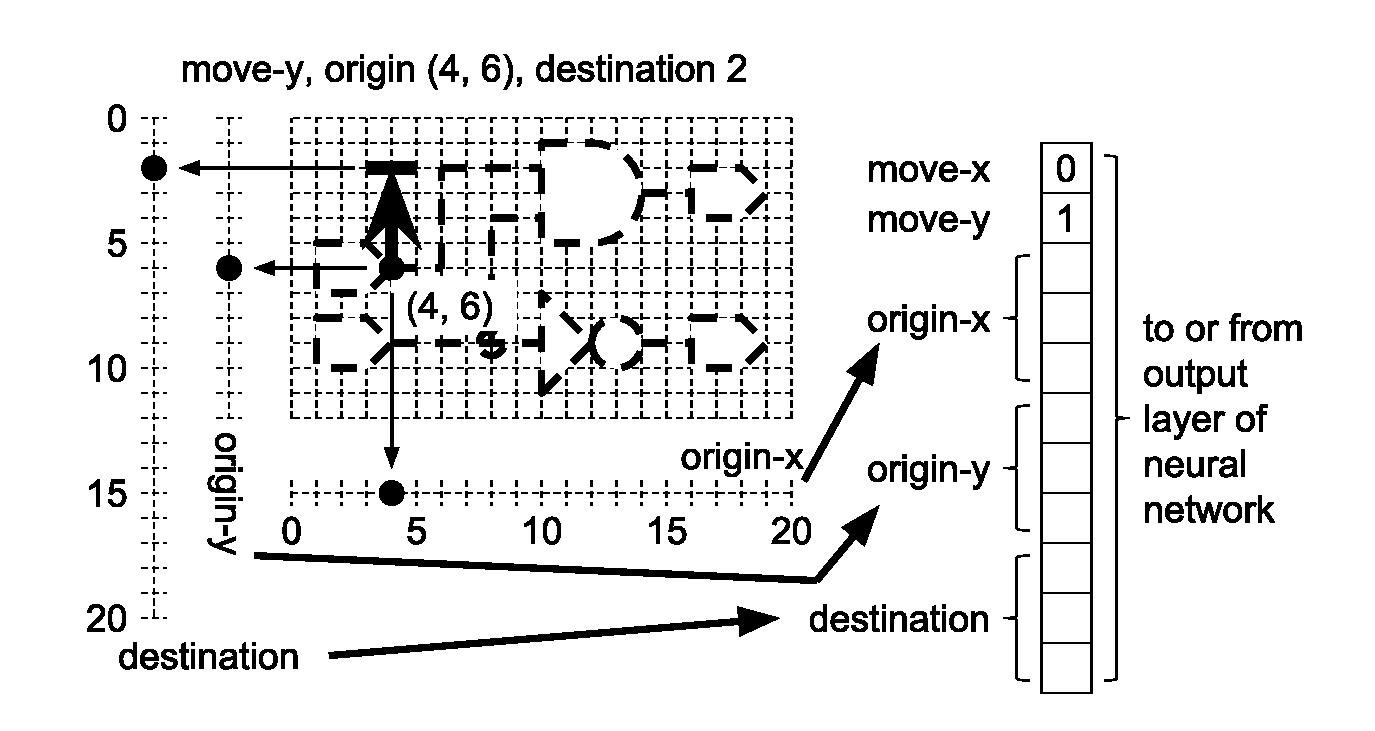
\includegraphics[width=\hsize]{output_encode_02.eps}
   \caption{a way to encode schematic for output vector of neural network}
   \label{fig:output_encode}
  \end{minipage}
 \end{center}
\end{figure}

\textbf{
The paper's graphics should have resolutions of 600dpi for monochrome,
300 dpi for grayscale, and 300 dpi for color. But, please do not include
too much high-resolution images or photos in your paper.
%%% Images or photos over 300dpi do not enhance the quality of your
%%% paper, but increase the size of the PDF file!
%%% Reduce the dpis of them as small as possible. 
} % Modified by N. Togawa 06/01/2005

\section{Helpful Hints}

\subsection{References}
List and number all references at the end of the paper. When reffering
to them in the text, type the corresponding reference number in the
parentheses as shown at the end of this sentence \cite{key}. Number
the citations consecutively. The sentence punctuation follows the
parentheses. Do not use ``Ref.\ \cite{baz}'' or
``reference \cite{baz}'' except at the beginning of a sentence.

\subsection{Footnotes}
Number the footnotes separately in superscripts. Place the actual
footnote at the bottom of the column in which it is cited. Do not put
footnotes in the reference list.

\subsection{Authors names}

Give all authors' names; do not use ``et al'' unless there are six
authors or more. Papers that have not been published, even if they have
been submitted for publication, should be cited as
``unpublished'' \cite{unpub}.  Papers that have been accepted for
publication should be cited as ``in press'' \cite{inpress}.
Capitalize only the first word in a paper title, except for proper nouns
and element symbols.

For papers published in translation journals, please give the English
citation first, followed by the original foreign language
citations \cite{trans}.

\subsection{Notice for \LaTeX\ users}

If you use \LaTeX\ to create your initial-submission paper, we recommend you
to use \texttt{dvipdfm} to produce PDF files from dvi files. If you cannot
use it, please use Type1 fonts instead of ugly Type3 fonts!

\section{Summary and Conclusions}

This template can be downloaded through the ASP-DAC 2018 web site
(http://www.aspdac.com/). If you have any problem, please contact ASP-DAC
2018 publication chair (jlee@unist.ac.kr).

%this is how to do an unnumbered subsection 
\section*{\sc Acknowledgements}
This article was written by referring to {\em ``Author's guide --
Preparation of Papers in Two-Column Format for VLSI Symposia on
Technology and Circuits''}, the {\em ``Preparation of Papers in
Two-Column Format for the Proceedings of the 32nd ACM/IEEE Design
Automation Conference''} written by Ann Burgmeyer, IEEE and {\em ``the
template for producing IEEE-format articles using \LaTeX''}, written by
Matthew Ward, Worcester Polytechnic Institute.

\begin{thebibliography}{9}
\footnotesize
\bibitem{key}
I. M. Author,
``Some related article I wrote,''
{\em Some Fine Journal}, vol. 17, pp. 1--100, 1987.

\bibitem{baz}
A. N. Expert,
{\em A Book He Wrote,}
His Publisher, 1989.

\bibitem{unpub}
M. Smith,
``Title of paper optional here,''
unpublished.

\bibitem{inpress}
K. Rose,
``Title of paper with only first word capitalized,''	% bug fixed by M. Imai
in press.

\bibitem{trans}
T. Murayama,
``Title of paper published in translation journals,''	% bug fixed by M. Imai
{\em Some English Journal}, vol. 17, pp. 1--100, 1995.	% bug fixed by M. Imai
({\em Original Foreign Journal, vol. 1, pp. 100-200, 1993}.)	% ditto

\end{thebibliography}
\end{document}
